%
% Copyright (c) 2011-2012, fortiss GmbH.
% Licensed under the Apache License, Version 2.0.
% 
% Use, modification and distribution are subject to the terms specified
% in the accompanying license file LICENSE.txt located at the root directory
% of this software distribution. A copy is available at
% http://chromosome.fortiss.org/.
%
% This file is part of CHROMOSOME.
%
% $Id$
%
% Author:
%         Michael Geisinger <geisinger@fortiss.org>
%

\section{Frequently Asked Questions}
\label{appx:faq}

\subsection{Technical Questions}

\subsubsection{How can I create a new component?}
\label{faq:create_component}

\xme comes with an application that can create template files for new components.
This application is called \verb|templateGenerator| and can be found in the \verb|bin/windows_x86|
subdirectory of the release package or built manually just like any other \xme example program (see Section~\ref{sec:example_helloworld} for hints).

The application will ask you for the component name, type as well as your name (for the author field)
and generate a header and a source file for the new component in the respective directory (compare Figure~\ref{fig:example_templateGenerator}).
Consider using one of the existing example applications for testing your new component if application, see Section~\ref{sec:example_chatcalculator}
for more information on how to embed a new component into an existing application.

\begin{figure}[htbp]
	\centering
	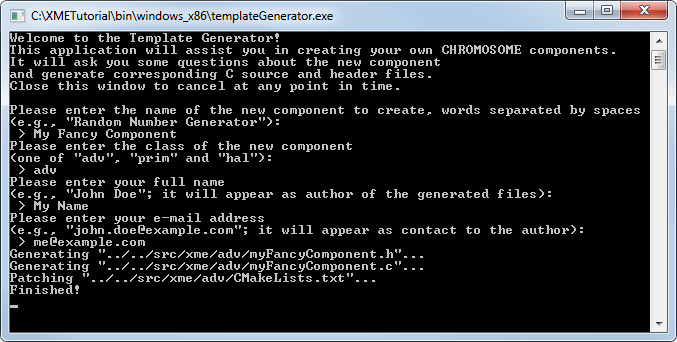
\includegraphics[scale=0.75]{figures/PNG/example_templateGenerator.png}
	\caption{\emph{Template Generator} in action.}
	\label{fig:example_templateGenerator}
\end{figure}

\subsubsection{How can I define a new topic?}

Topic identifiers are simple numbers with associated semantics.
The \verb|xme_core_topic_t| type defined in file \verb|<XME_ROOT>/xme/core/topic.h| declares some generic topic identifiers.
Topic numbers in the range between zero and \verb|XME_CORE_TOPIC_USER|-1 are reserved for internal use.
This means that you can define a new topic by using an arbitrary number larger or equal to \verb|XME_CORE_TOPIC_USER|.

Note that there is currently no mechanism in place for checking that the same topic identifiers are always used for the same type of data.
Be aware that other people in the same network might use the same topic identifiers for their data.
We plan to put a mechanism in place for avoiding this issue in future versions of \xme.

\subsubsection{How can I port \xme to my own target platform?}

The current release of \xme supports only Windows.
However, we are in the process of developing platform support layers for other platforms.
These include Linux, medium-sized microcontroller platforms like ARM Cortex M3 (e.g., as central control units)
as well as low-end microcontrollers like Atmel AVR (e.g., for sensor networks).
Upcoming releases of \xme will ship with the respective functionality.

If you favorite platform is not on this list, there are multiple options:
\begin{enumerate}
	\item You can suggest \xme to be ported onto your platform.
		If your application is of high relevance, we might indeed port \xme to that platform.
	
	\item You can contribute to the development of \xme and have your platform supported as a target platform.
	
	\item You can take the \xme source code and implement the respective platform support without revealing the source code.
		Our license model permits this (see also Appendix~\ref{appx:license}).
\end{enumerate}

\subsection{Conceptual Questions}

\subsubsection{How do you want to implement semantic aspects?}

Current middleware technology lacks semantic integration.
We are using a data-centric design, where we describe the data with an ontology.
If several domains are involved, there might be the necessity to map between the domain-specific ontologies.
This must be done manually, but can be reused (and must therefore be done only once).

% Thoughts (CB):
% Actually I am not sure, whether we really need a full-blown ontology.
% Most probably a list of available data classes is enough.
% In addition a good structuring (e.g. in the automotive area according to the different domains) might be useful.

\subsubsection{How do you specify extra-functional requirements?}

We use meta-data to describe concrete data sources.
Examples for meta-data are accuracy, confidence level, age.
In addition, we want to use application patterns to describe the extra-functional properties of concrete applications.

\subsubsection{How do you guarantee extra-functional requirements?}

We focus on implementations that can easily guarantee these requirements (e.g., time-triggered execution).
If we have more flexible protocols, we have two options: either we cannot guarantee requirements or we have to be more pessimistic.

% Thoughts (CB):
% Our main advantage is that we know the requirements (even at run-time).
% In todays systems, the only thing that the system knows at run-time is the configuration that was derived by the requirements.
% However, the concrete motivation for a specific solution is not available at run-time.
% Hence, the system cannot properly react if something goes wrong (good example: run-time monitoring of assumptions is typically not done).
